\chapter{\TwoDContractionMap to \EOPL}
\label{sec:twoDContractionMapToEOPL}
In this chapter, we reduce a slightly weaker variant of \CM to \EOPL. Aside from providing further evidence for the \CLS-hardness of \EOPL, the technique we introduce in this reduction is of independent interest and we believe may be applicable to reducing \CM, \MMCM, or \MBanach to \EOPL, which would show \CLS-completeness of \EOPL in the latter two cases.

We restate the definition of \EOPL here for convenience:

\begin{definition}[\EOPL]
\label{def:EOPL2}
Given Boolean circuits $S,P : \Set{0,1}^n \to \Set{0,1}^n$ such that $P(0^n) =0^n\neq S(0^n)$ and a Boolean circuit $V: \Set{0,1}^n \to \Set{0,1,\dotsc,2^m - 1}$ such that $V(0^n) = 0$ find one of the following:
\begin{enumerate}[label=(R\arabic*)]
\item A point $x \in \Set{0,1}^n$ such that $S(P(x)) \neq x \neq 0^n$ or $P(S(x)) \neq x$. \label{eopl2:eol}
\item A point $x \in \Set{0,1}^n$ such that $x \neq S(x)$, $P(S(x)) = x$, and $V(S(x)) - V(x) \leq 0$. \label{eopl2:bad_potential}
\end{enumerate}
\end{definition}


The variant of \CM (Definition~\ref{def:contractionmap}) we will consider here differs from \CM in that the domain and range of the map is $[0,1]^2$ instead of $[0,1]^3$, and in that the norm under consideration is required to be a $p$-norm.
\begin{definition}[\TwoDContractionMap] 
  \label{def:2DContractionMap}
We are given as input an arithmetic circuit computing $f: [0,1]^2\to [0,1]^2$,
a choice of $p$-norm $\Norm{\cdot}_p$, constants \mbox{$c \in (0,1)$}
and $\delta > 0$. It is asserted that $f$ is $c$-contracting with respect to $\Norm{\cdot}_p$.
The goal is to find
\begin{enumerate}[label=(E\arabic*)]
\item a point $x\in [0,1]^2$ such that $\Norm{f(x),x}_p \leq \delta$, \label{2dcm:fixpoint}
\item or two points $x,y\in [0,1]^3$ such that $\Norm{f(x) - f(y)}_p/\Norm{x-y}_p > c$. \label{2dcm:violation}
\end{enumerate}
\end{definition}

The observation underlying the reduction is that applying the standard reduction from the computational version of Brouwer's Fixed-Point Theorem to Sperner's Lemma in the special case of contraction maps results in instances of Sperner's Lemma in which the the given Sperner path has a very special structure. This structure then allows us to assign a consistent potential function to the vertices of the \PPAD graph created in the reduction from Sperner's Lemma to \EOL.

The precise version of the Sperner problem we will use is the following, due to Papadimitriou \cite{papadimitriou1994complexity}:
\begin{definition}[\Sperner] 
  \label{def:Sperner}
  We are given as input an algorithm
  \[\mycolor: \Set{0/n,1/n,\dotsc,n/n}^2 \to \Set{\Blue, \Red, \Yellow}\] that computes a color for the vertices of an $n\times n$ subdivision of the unit square in polynomial-time (in the binary representation of $n$). The coloring given by the algorithm satisfies the following constraints:
  \begin{itemize}
  \item $\mycolor(0, 0) = \Yellow$, $\mycolor(1, 0) = \Blue$, and $\mycolor(0, 1) = \Red$.
  \item If $x_1 = 1$ or $x_2 = 1$, $\mycolor(x_1,x_2) \in \Set{\Blue, \Red}$.
  \item If $x_1 = 0$, $\mycolor(x_1,x_2) \in \Set{\Red, \Yellow}$.
  \item If $x_2 = 0$, $\mycolor(x_1,x_2) \in \Set{\Blue, \Yellow}$.
  \end{itemize}

  The goal is to find a triangle $x,y,z$ formed by three corners of the a $1/n$-side length square such that \[\Set{\mycolor(x),\mycolor(y),\mycolor(z)} = \Set{\Blue,\Red,\Yellow}\text{.}\] Such a triangle is called a \emph{trichromatic} triangle.
\end{definition}

Such a triangle is guaranteed to exist for any \emph{legal} coloring where a legal coloring is one that satisfies the above constraints, by Sperner's lemma \cite{papadimitriou1994complexity}.

To reduce \Sperner to \EOL, we need to take the coloring given by $\mycolor$ and add a single square-width boundary around all of $[0,1]^2$, with a fixed coloring (illustrated in Figure \ref{fig:withAndWithoutBorder} and included in the reduction below) to obtain another coloring \[\mycolor_1 : \Set{-1/n,0/n,\dotsc,(n+1)/n}^2 \to \Set{\Blue, \Red, \Yellow}\text{.}\]  Since our interest is in the final \EOPL instance, we won't present a borderless coloring and then add a border, but rather we'll directly present the final coloring with a border.

\section{The Reduction}
We start with an instance $\CI$ of $\TwoDContractionMap$ consisting of $f$, $\Norm{\cdot}_p$, $c$, and $\delta$, We first set $\e \triangleq \delta/2^{2+1/p}$, and then set $n \triangleq 2^{\Ceil{\ln(1/\e)}} \geq \Ceil{1/\delta}$. We now define a domain $\Dom$ corresponding to a discretization of the unit square $[0,1]^2$ with a uniform thickness boundary added around it,
\[\Dom = \Set{-1/n,0/n,1/n,\dotsc,(n-1)/n,n/n,(n+1)/n}^2\text{.}\]

Let $\DomInt = \Set{0/n,\dotsc,n/n}^2 = \Dom\cap [0,1]^2$ be the points of $\Dom$ contained in the unit square.

We'll define our \EOPL instance $\CE$ over triangles formed by triplets from $\Dom$.  Particularly our vertex set will consist of triangles defined by triples
  \[z^0,z^1,z^2\] where either $z^1 = z^0 + (1,0)/n$ and $z^2 = z^0 - (0, 1)/n$ or $z^1 = z^0 + (1,-1)/n$ and $z^2 = z^0 - (1,0)/n$. These are triangles where the hypotenuse goes from top-left to bottom-right, and they are presented by listing the vertices in clockwise order. Let $\Delta(\Dom)$ denote the set of such triangles where $z^0,z^1,z^2 \in \Dom$, and let $\Delta(\DomInt) \subseteq \Delta(\Dom)$ denote the subset of $\Delta(\Dom)$ where $z^0,z^1,z^2 \in \DomInt$. We set $\vert = \Delta{\Dom}$.\footnote{To be fully formal, we would need to encode such triplets as binary strings. The obvious encoding of triples as the concatenation of the binary representations of the vertices would introduce dummy vertices which we could handle by making sure all dummy vertices were isolated with self-loops. See \ref{sec:PLCPtoEOPL} for a reduction in which we do exactly this.}

  We'll start by constructing a coloring of $\Dom$ that consists of a fixed boundary coloring surrounding a legal coloring of $\DomInt$. For any point $x \in \DomInt$ $\mycolor(x)$ will depend on the direction of the displacement $f(x) - x$; Figure \ref{fig:colorMap} illustrates the particular coloring used. Points in $\Dom\setminus \DomInt$ will be colored according to the canonical border coloring for Sperner's Lemma. For any point $z \in [0,1]^2$, let $\theta(z)$ denote the clockwise angle between the positive $x$-axis and the vector $z$. An example coloring without a border, and one with a border are provided in Figures \ref{fig:withoutBorder} and \ref{fig:withBorder}, respectively. Figure \ref{fig:displacement} contains example with displacement vectors drawn at each point.

  \begin{figure}
    \centering
    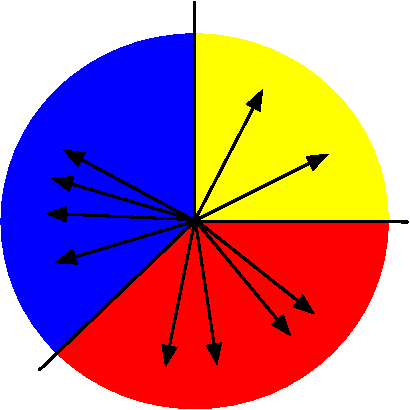
\includegraphics[scale=0.5]{ColorMap}
    \caption{The colors assigned to each displacement direction. Points with displacements along the black lines between regions will be colored so as to ensure the boundary satisfies the requirements of Sperner's Lemma.}
    \label{fig:colorMap}
  \end{figure}

  \begin{figure}
    \centering
    \begin{subfigure}[h]{0.7\textwidth}
      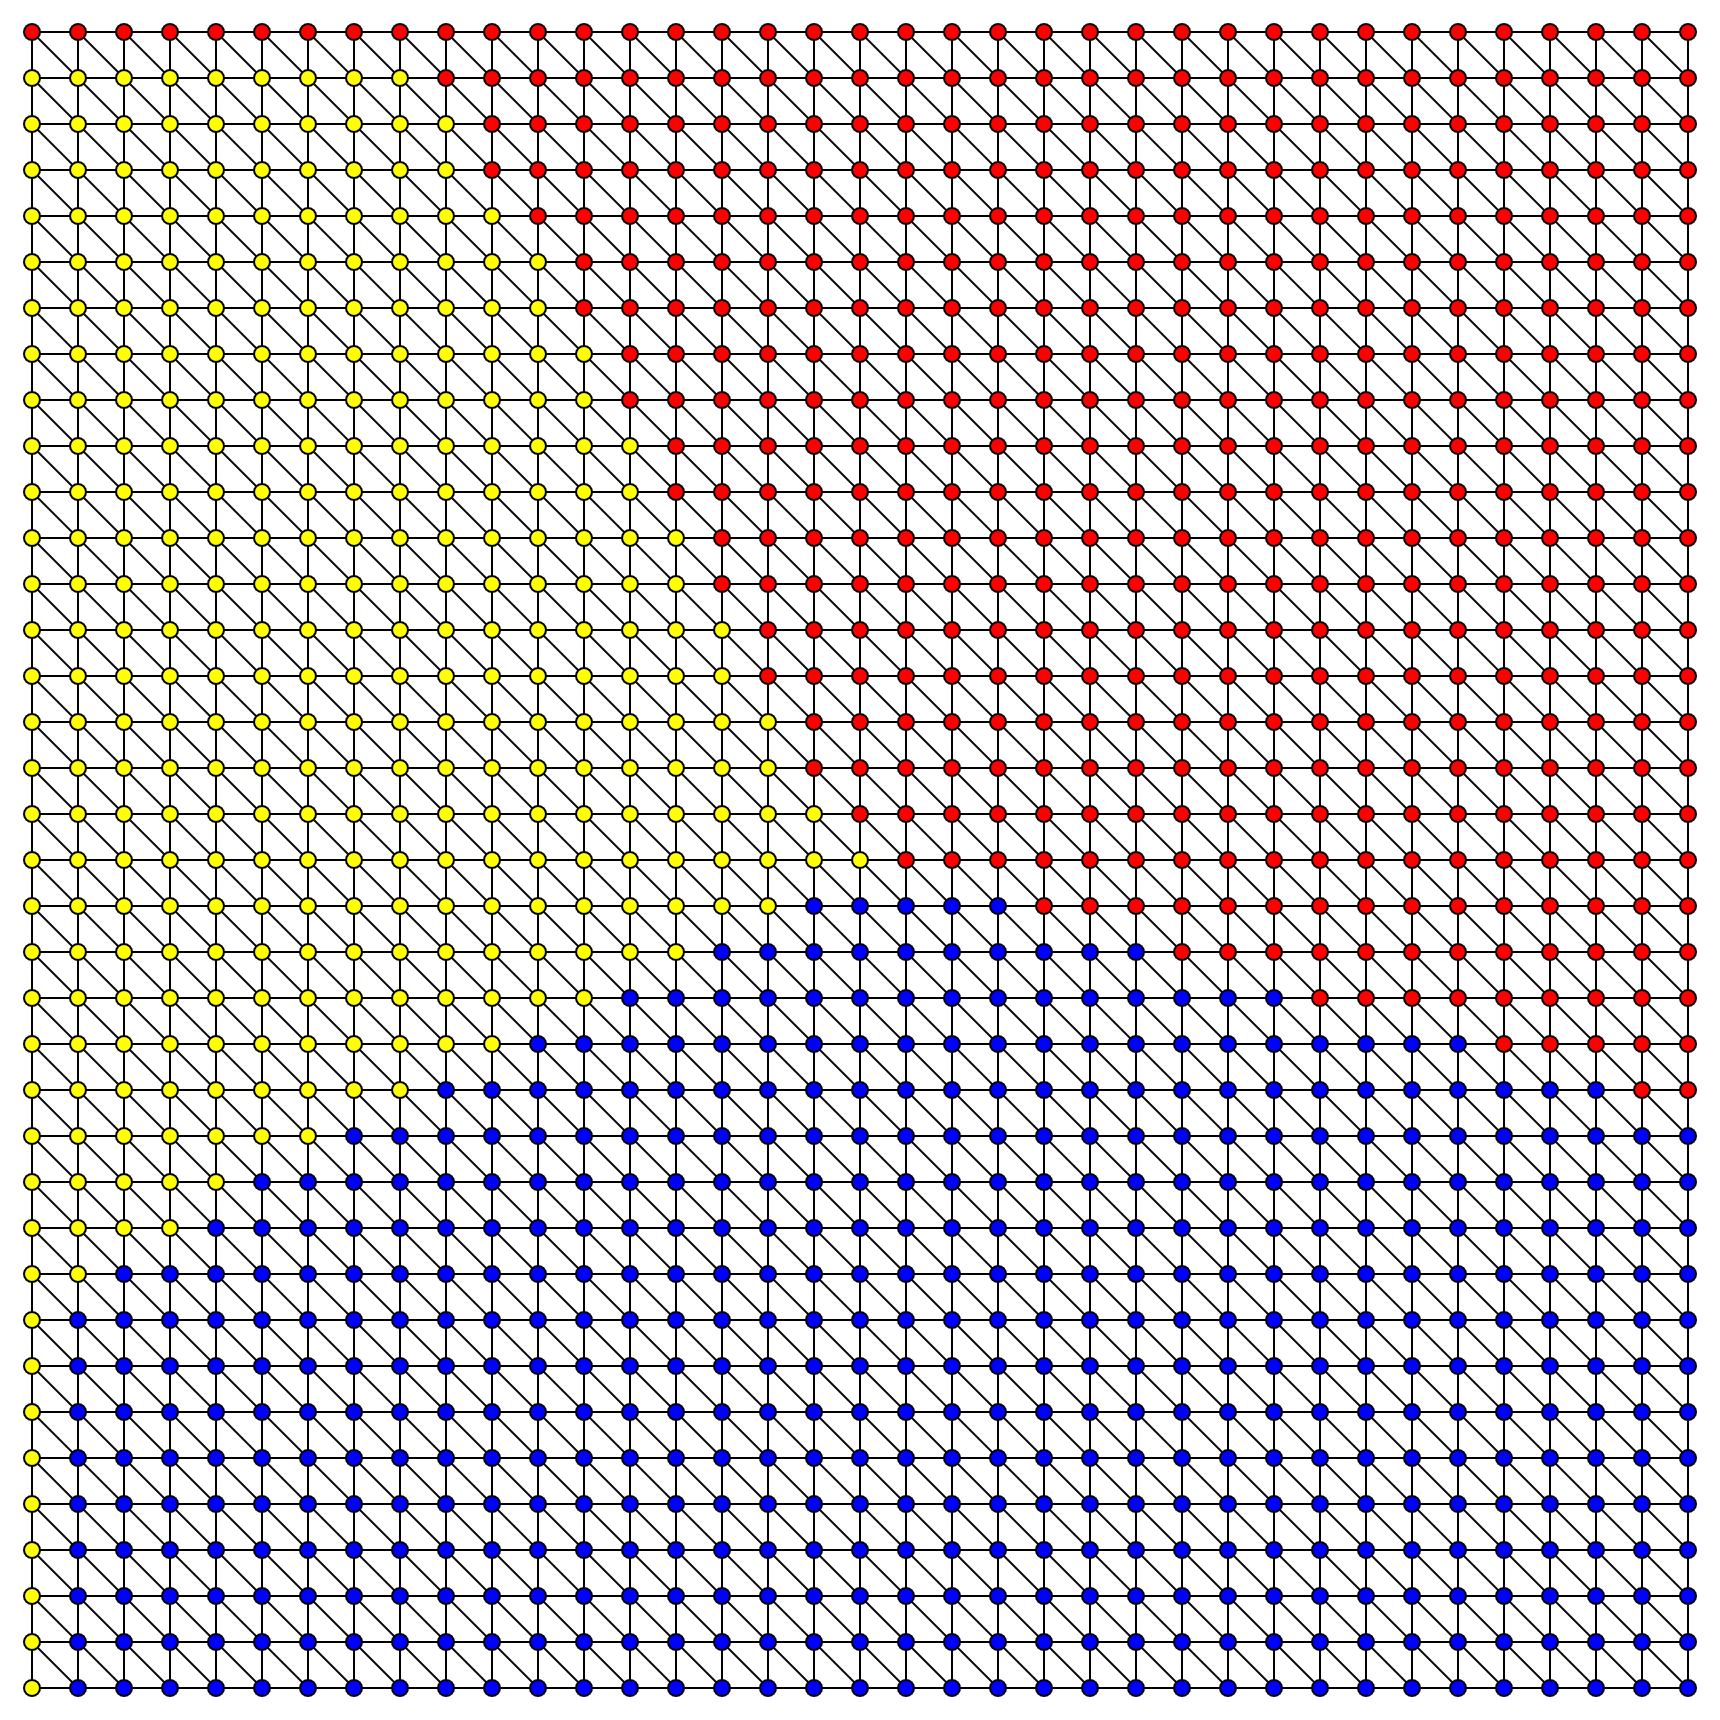
\includegraphics[width=\textwidth]{ContractionToEOPL_example1_WithoutBorder}
      \caption{A coloring for a contraction map without an added border.}
      \label{fig:withoutBorder}
    \end{subfigure}
    \begin{subfigure}[h]{0.7\textwidth}
      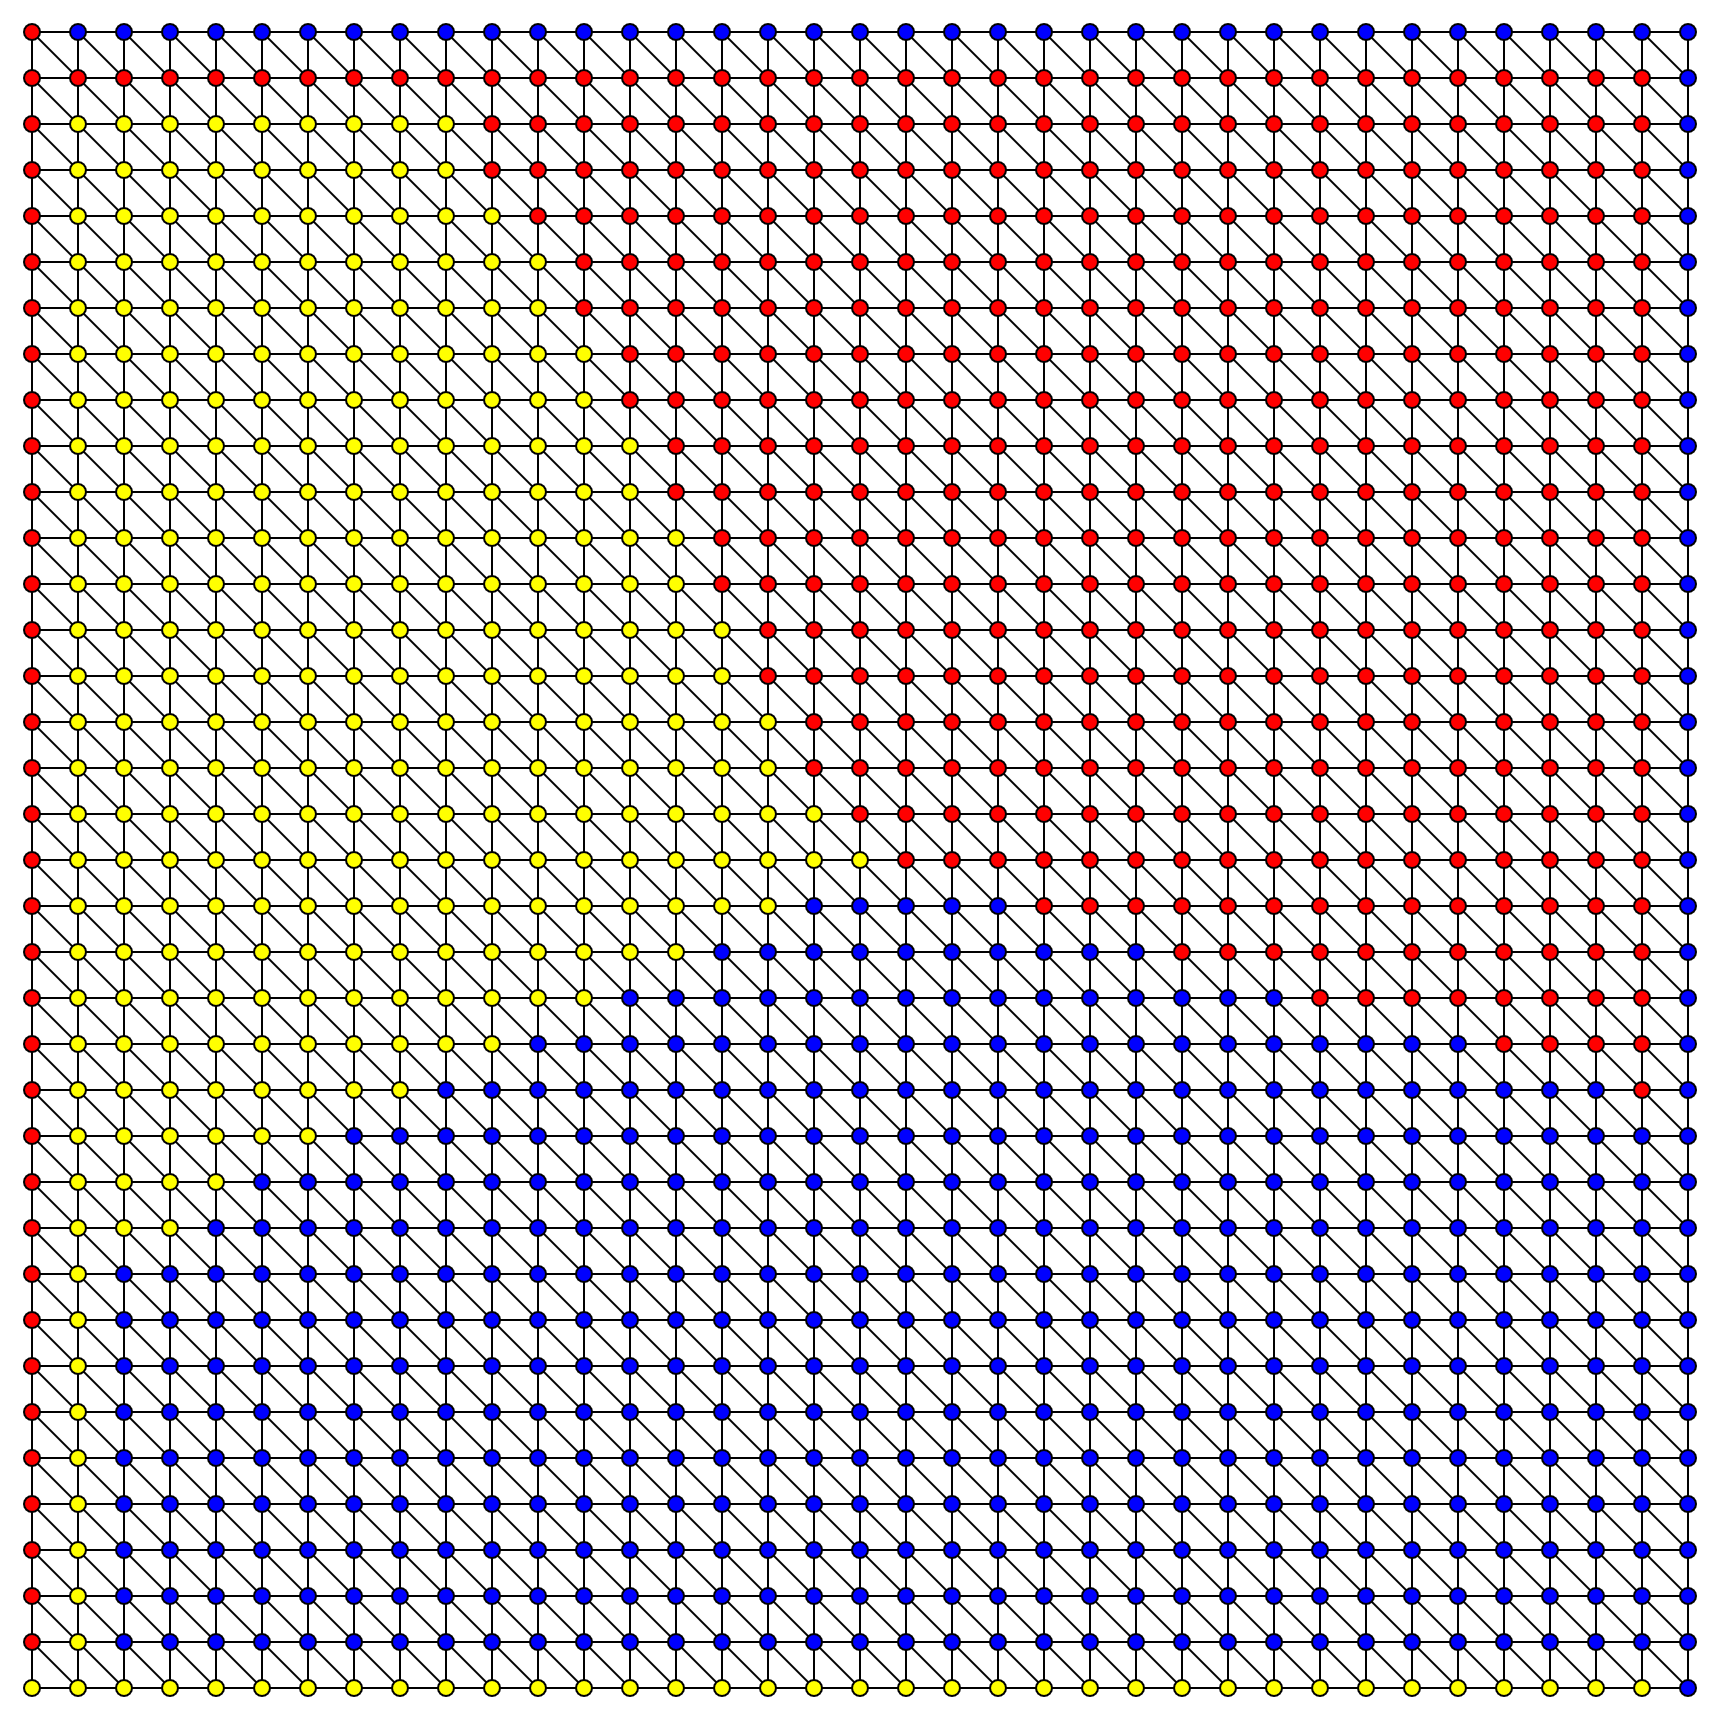
\includegraphics[width=\textwidth]{ContractionToEOPL_example1_WithBorder}
      \caption{A coloring for a contraction map with an added border.}
      \label{fig:withBorder}
    \end{subfigure}    
    \caption{Example colorings for a contraction map with and without an added border.}
    \label{fig:withAndWithoutBorder}
  \end{figure}


  \begin{figure}[h] 
    \caption{Coloring for a contraction map with displacement vectors shown at each non-boundary point.}
    \centering
    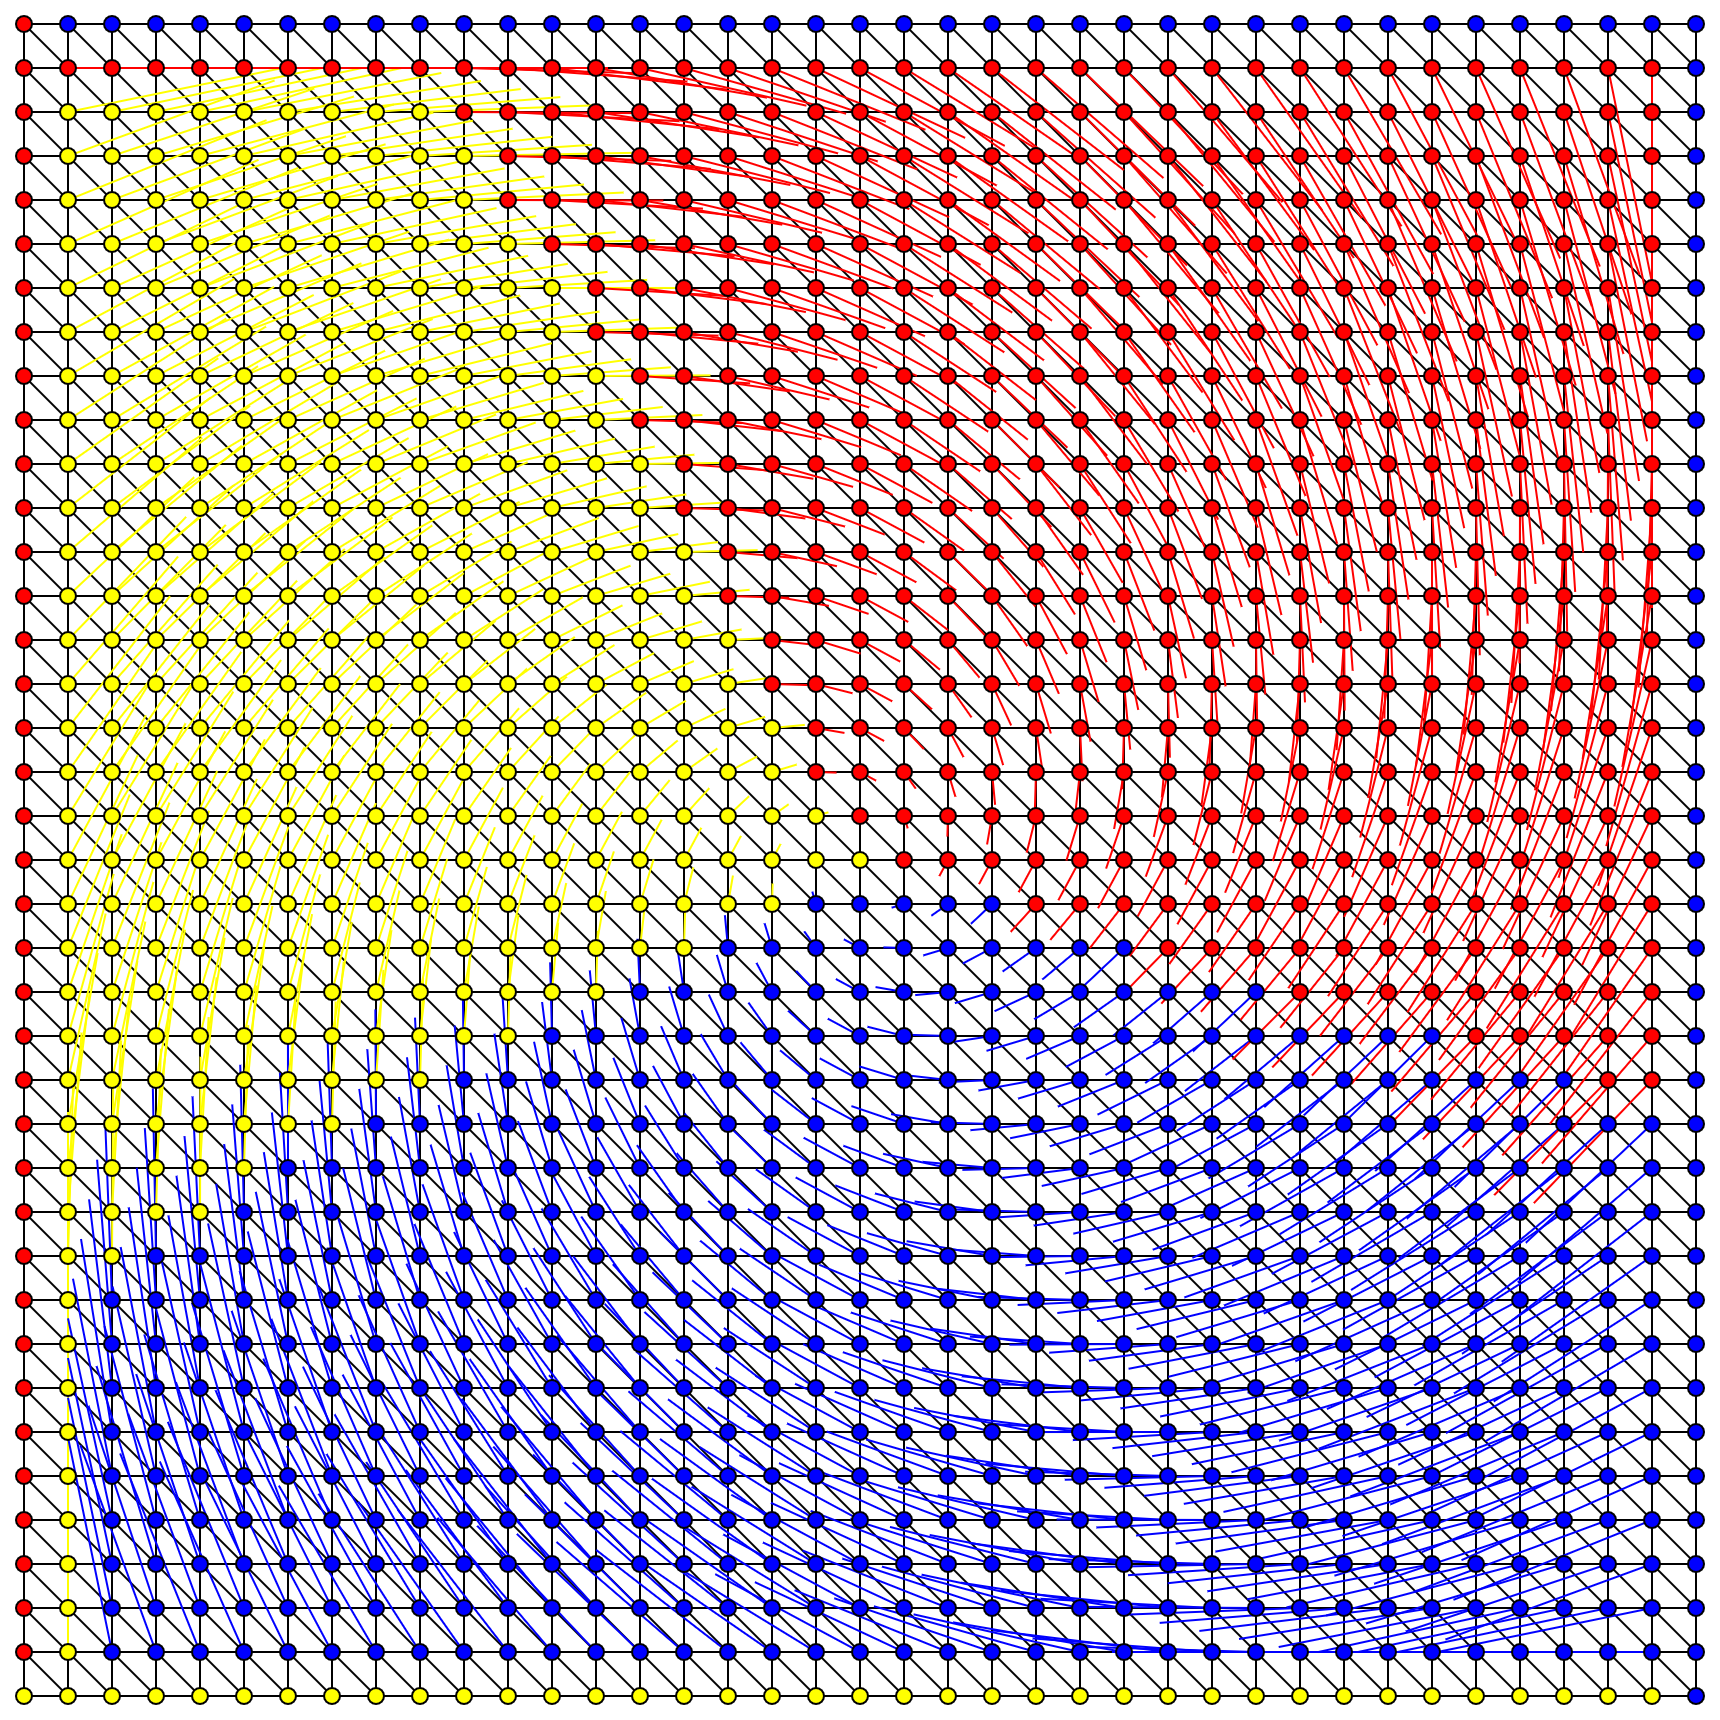
\includegraphics[width=0.7\textwidth]{ContractionToEOPL_example1_displacement}
    \label{fig:displacement}
  \end{figure}

  We assign colors from $\Set{\Yellow, \Blue, \Red}$ as follows:
  \begin{algo}
    $\mycolor(z)$:\+
    \\ \AlgoComment{Boundary Coloring}
    \\ \IfB $z_1 = -1/n$ \textbf{and} $z_2 \neq -1/n$:\+
    \\   \ReturnB $\Red$\-
    \\ \ElseIfB $z_2 = -1/n$ \textbf{and} $z_1 \neq (n+1)/n$:\+
    \\   \ReturnB $\Yellow$\-
    \\ \ElseIfB $z_2 = (n+1)/n$ \textbf{or} $z_1 = (n+1)/n$:\+
    \\   \ReturnB $\Blue$\-
    \\
    \\ \AlgoComment{Interior Coloring}
    \\ \IfB $\theta(f(z) - z) \in [0, \pi/2]$:\+
    \\   \IfB $z_1 = 1$:\+
    \\     \ReturnB $\Blue$\-
    \\   \ElseIfB $z_2 = 1$:\+
    \\     \ReturnB $\Red$\-
    \\   \ElseB:\+
    \\     \ReturnB $\Yellow$\-\-
    \\ \ElseIfB $\theta(f(z) - z) \in (\pi/2, 5\pi/4)$:\+
    \\   \ReturnB $\Blue$\-
    \\ \ElseIfB:\+
    \\   \ReturnB $\Red$\-\-
  \end{algo}

  Let $\mycolor\restr_{\DomInt} : \DomInt \to \Set{\Blue, \Red, \Yellow}$ denote the restriction of $\mycolor$ to $\DomInt$. The following lemma is immediate:
  \begin{lemma}
    $\mycolor\restr_{\DomInt}$ is a legal coloring of $\DomInt$ for any function $f: [0,1]^2\to [0,1]^2$
  \end{lemma}

  Moreover, the border coloring doesn't introduce any trichromatic triangle. As a result, we have that
  \begin{lemma}
    There exists a trichromatic triangle $x,y,z$ under $\mycolor$ where $x,y,z\in \DomInt$, and there are no trichromatic triangles containing vertices in $\Dom\setminus \DomInt$.
  \end{lemma}

  Furthermore, any trichromatic triangle entirely contained in $\DomInt$ gives a solution to the starting instance $\CI$. This can be seen in the folllowing lemma, part of which appears in a similar form in \cite{scarf1967approximation}:

  \begin{lemma}
      \label{lemma:TrichromaticTriangles}
    If $z^Y,z^R,z^B \in \Delta(\DomInt)$ are yellow, red, and blue vertices, respectively, of a trichromatic triangle (not necessarily in clockwise order), then either $z^Y$ is a solution of type \ref{2dcm:fixpoint} or two of the vertices in the triangle give a solution of type \ref{2dcm:violation}.
  \end{lemma}
  \begin{proof}
    By construction, $(f(z^Y) - z^Y)_1 (f(z^B) - z^B)_1 \leq 0$ and $(f(z^Y) - z^Y)_2 (f(z^R) - z^R)_2 \leq 0$.
    If $f$ is $c$-contracting, then we have 
    \begin{align*}
      \Abs{(f(z^Y) - z^Y)_1} &\leq \Abs{(f(z^Y) - z^Y)_1 - (f(z^B) - z^B)_1}\\
                             &= \Abs{(f(z^Y) - f(z^B))_1 + (z^B - z^Y)_1}\\
                             &\leq \Abs{(f(z^Y) - f(z^B))_1} + \Abs{(z^Y - z^B)_1}\\
                             &\leq \Norm{(f(z^Y) - f(z^B))_1} + \Norm{(z^Y - z^B)}\\
                             &\leq (c+1)\Norm{(z^Y - z^B)_1}\\
                             &\leq 4\e\\
                             &\leq \delta/2^{1/p}
    \end{align*}  and by an analogous argument, we have
    \[ \Abs{(f(z^Y) - z^Y)_2} \leq \delta/2^{1/p}\text{.} \]

    If either of these fails to hold, then the corresponding pair of points is a solution of type \ref{2dcm:violation}.

    If both hold, then we have
    \begin{align*}
      \Norm{f(z^Y) - z^Y}_p &= \Paren{\Abs{(f(z^Y) - z^Y)_1}^p + \Abs{(f(z^Y) - z^Y)_2}^p}^{1/p} \\
                          &\leq \Paren{\delta^p/2 + \delta^p/2}^{1/p}\\
                          &\leq \delta
    \end{align*} and $z^Y$ is a solution of type \ref{2dcm:fixpoint}.
  \end{proof}

  Before defining the \EOPL instance from this coloring, we make the key observation needed to get a valid potential function: If $f$ is a valid contraction map (with any constant $c < 1$), there is no yellow point above a red point, i.e., there is no pair $z^Y,z^R \in D$ with $z^R = z^Y - (0,k/n)$ with $\mycolor(z^Y) = \Yellow$ and $\mycolor(z^R) = \Red$ for any $k$. 

  \begin{lemma} \label{lemma:YellowAboveRed}
    If $z^Y, z^R \in D$ with $z^R = z^Y - (0,1)/n$ such that $\mycolor(z^Y) = \Yellow$ and $\mycolor(z^R) = \Red$, then $\Norm{f(z^Y) - (z^R)}_p \geq \Norm{z^Y - z^R}_p$, and $f$ is not a contraction map.
  \end{lemma}

  \begin{proof}
    Let $z^Y$ and $z^R$ be as in the statement. By our border coloring, it cannot be the case that $z^Y_1 = -1$, $z^Y_1 = n+1$, or $z^Y_2 = n+1$. Nor can $z^R_2 = -1$. Thus, both $z^R$ and $z^Y$ must have been colored according to $\theta^Y = \theta(f(z^Y) - z^Y)$ and $\theta^R = \theta(f(z^R) - z^R)$. By construction, we have $\theta^Y \in [0,\pi/2]$ and $\theta^R \in [5\pi/4,2\pi)$. So \[ (f(z^Y) - z^Y)_2 (f(z^R) - z^R)_2 \leq 0 \] and we have
    \begin{align*}
      \Norm{f(z^R) - f(z^Y)}_p &\geq \Abs{(f(z^R) - f(z^Y))_2} \\
                               &> \Norm{z^R - z^Y}_p
    \end{align*}

    so $z^R$ and $z^Y$ are witnesses to $f$ not being $c$-contracting (or contracting at all).
  \end{proof}

  \begin{corollary} \label{corollary:LeftEdgeIsSolution}
    If $z^Y$ and $z^R$ are vertices of a triangle in $\Delta(\DomInt)$ with $\mycolor(z^Y) = \Yellow$, $\mycolor(z^R) = \Red$, and $z^Y = z^R + (0,1/n)$, then the pair $(z^Y,z^R)$ is a solution of type \ref{2dcm:violation} for $\CE$.
  \end{corollary}

  We now will construct the \EOPL instance from this coloring. Intuitively, two triangles will be adjacent if they share an edge with one $\Red$ endpoint and one $\Yellow$ endpoint. We will orient the edges of the \EOPL graph so that there is an edge from $(z^0, z^1, z^2)$ to $(w^0, w^1, w^2)$ if facing the shared $\Red$-$\Yellow$ from a point inside $(z^0, z^1, z^2)$, the $\Red$ endpoint is to the left of the $\Yellow$ endpoint. Equivalently, the edge is oriented in this way if the $\Red$ vertex immediately preceeds the $\Yellow$ vertex in a clockwise enumeration of the vertices $z^0,z^1,z^2$ (perhaps beginning with $z^1$ or $z^2$). 

  Lemma~\ref{lemma:YellowAboveRed} now implies that the \EOPL graph will never have edges from right to left if $f$ is a contraction map, since edges from right to left have a yellow top-endpoint and a red bottom-endpoint. By Corollary~\ref{corollary:LeftEdgeIsSolution}, both triangles sharing such an edge give solutions to $\CE$, so we modify the graph to make the left triangle the start of its path, and the right triangle the end of its path.

  \begin{algo}
    $\Succ(z^0,z^1,z^2)$:\+
    \\ \IfB $\exists i,j$ with $j = i + 1 \pmod{3}$ such that $\mycolor(z^i) = \Red$ and $\mycolor(z^j) = \Yellow$:\+
    \\   \IfB $z^1 = z^0 + (1,0)/n$:\quad\AlgoComment{Top-right corner triangle\+  }  
    \\     \IfB $i = 0$:\+
    \\       \ReturnB $z^0+(0,1)/n,z^1,z^0$\quad\AlgoComment{Successor is above}\-
    \\     \ElseIfB $i = 1$:\+
    \\       \ReturnB $z^1,z^2 + (1,0)/n,z^2$\quad\AlgoComment{Successor is to the right}\-
    \\     \ElseB:\quad\AlgoComment{Successor is below and to the left}\+
    \\       \ReturnB $z^0,z^2,z^0 - (0,1)/n$\-\-
    \\   \ElseB:\quad\AlgoComment{Bottom-left corner triangle}\+
    \\     \IfB $i = 0$:\quad\AlgoComment{Successor is above and to the right}\+
    \\       \ReturnB $z^0,z^0+(1,0)/n,z^1$\-
    \\     \ElseIfB $i = 1$:\quad\AlgoComment{Successor is below}\+
    \\       \ReturnB $z^2,z^1,z^1-(0,1)/n$\-
    \\     \ElseB: \quad\AlgoComment{We have a violation of contraction by Lemma \ref{lemma:YellowAboveRed}}\+
    \\       \ReturnB $z^0,z^1,z^2$\quad\AlgoComment{Make this the end of a line}\-\-\-
    \\ \ReturnB $z^0,z^1,z^2$\quad\AlgoComment{Make a self-loop if no leaving edge}
  \end{algo}
    
  \begin{algo}
    $\Pred(z^0,z^1,z^2)$:\+
    \\ \IfB $\exists i,j$ with $j = i + 1 \pmod{3}$ such that $\mycolor(z^i) = \Yellow$ and $\mycolor(z^j) = \Red$:\+
    \\   \IfB $z^1 = z^0 + (1,0)/n$:\quad // Top-right corner triangle\+    
    \\     \IfB $i = 0$:\quad Predecessor is above\+
    \\       \ReturnB $z^0+(0,1)/n,z^1,z^0$\-
    \\     \ElseIfB $i = 1$: \quad// We have a violation of contraction by Lemma \ref{lemma:YellowAboveRed}\+
    \\       \ReturnB $z^0,z^1,z^2$ \quad// Make this the start of a line\-
    \\     \ElseB:\quad // Predecessor is below and to the left\+
    \\       \ReturnB $z^0,z^2,z^0 - (0,1)/n$\-\-
    \\   \ElseB:\quad // Bottom-left corner triangle\+
    \\     \IfB $i = 0$:\quad // Predecessor is above and to the right\+
    \\       \ReturnB $z^0,z^0+(1,0)/n,z^1$\-
    \\     \ElseIfB $i = 1$:\quad // Predecessor is below\+ 
    \\       \ReturnB $z^2,z^1,z^1-(0,1)/n$\-
    \\     \ElseB:\quad // Predecessor is to the left\+
    \\       \ReturnB $z^0-(1,0)/n,z^0,z^2$\-\-\-
    \\ \ReturnB $z^0,z^1,z^2$ \quad// Make a self-loop if no entering edge
  \end{algo}
  
  Having removed all right-to-left edges from the \EOPL graph, we'll be able to upper bound the length of the Sperner path starting in the bottom left triangle to get to any triangle in $\Delta(\Dom)$. We can then use this upper bound to assign potentials to each triangle that are guaranteed to be greater than any potential in a previous triangle along that path.

  We will set a triangle's potential to the length of the longest path that could have possibly led to this triangle. To that end, the potential of a triangle $z^0,z^1,z^2$ will be the sum of the number of triangles to the left of this one, $2(n+2)(z^0_1 + 1)$, and the number of triangles ``before'' this one with top-left corners in the same column as $z^0$. This is slightly trickier than it sounds. 
  Counting the number of triangles ``before'' the triangle in question is done by determining whether the path in this column is going up or down so that we can start counting from the bottom or top, respectively. To do this we first check whether the successor of this triangle gives us enough information to determine the direction. If not, we check the predecessor. If after doing this we still don't have enough information to determine the direction of the path in this column, then this triangle must be an isolated vertex, and we can give it a dummy potential value of $0$ (which doesn't introduce solutions since any such vertex will have a self-loop).

One additional complication arises when we observe that there are two triangles sharing the same top-left corner, and we need to account for this when counting triangles before the current triangle. 
  \begin{algo}
    $\Value(z^0,z^1,z^2)$:\+
    \\  $(s^0,s^1,s^2) \gets \Succ(z^0,z^1,z^2)$
    \\  $(p^0,p^1,p^2) \gets \Pred(z^0,z^1,z^2)$
    \\  \IfB $(z^0,z^1,z^2) \neq (s^0,s^1,s^2)$:\quad\AlgoComment{Has a possible successor}\+
    \\    \IfB $z^2 = z^0 - (0,1)/n$:\quad\AlgoComment{Bottom-left corner triangle}\+
    \\      \IfB $s^0 = z^0$:\quad\AlgoComment{Successor across the diagonal}\+
    \\        \ReturnB $2(n+2)(z^0_1 + 1) + 2z^0_2$\-
    \\      \ElseB:\quad\AlgoComment{Successor is below, since there are no successors to the left}\+
    \\        \ReturnB $2(n+2)(z^0_1 + 1) + 2(n+1-z^0_2) + 1$\-\-
    \\    \ElseB:\quad\AlgoComment{Top-right corner triangle}\+
    \\      \IfB $s^0 = z^0$:\quad\AlgoComment{Successor is across the diagonal}\+
    \\        \ReturnB $2(n+2)(z^0_1 + 1) + 2(n+1-z^0_2)$\-
    \\      \ElseIfB $s^2 = z^0$:\quad\AlgoComment{Successor is above}\+
    \\        \ReturnB $2(n+2)(z^0_1 + 1) + 2z^0_2 + 1$\-\-\-
    \\ \AlgoComment{Either has no successor or is top-right corner triangle with successor to the right}
    \\  \IfB $(z^0,z^1,z^2) \neq (p^0,p^1,p^2)$:\quad\AlgoComment{Has a possible predecessor}\+
    \\    \IfB $z^2 = z^0 - (0,1)/n$:\quad\AlgoComment{Bottom-left corner triangle, must not have had successor}\+
    \\      \IfB $p^0 = z^0$:\quad\AlgoComment{Predecessor is across the diagonal}\+
    \\        \ReturnB $2(n+2)(z^0_1 + 1) + 2(n+1-z^0_2) + 1$\-
    \\      \ElseB:\quad\AlgoComment{Predecessor to the left with no successor or predecessor below}\+
    \\        \ReturnB $2(n+2)(z^0_1 + 1) + 2z^0_2$\-\-
    \\    \ElseB:\quad\AlgoComment{Top-right corner triangle with no successor or right successor}\+
    \\      \IfB $p^2 = z^0$:\quad\AlgoComment{Predecessor is above}\+
    \\        \ReturnB $2(n+2)(z^0_1 + 1) + 2(n+1-z^0_2)$\-
    \\      \ElseB:\quad\AlgoComment{Predecessor across the diagonal}\+
    \\        \ReturnB $2(n+2)(z^0_1 + 1) + 2z^0_2 + 1$\-\-\-
    \\  \ReturnB $0$\quad\AlgoComment{Isolated triangle, in a self-loop}. 
  \end{algo}

  In Figure \ref{fig:potentials}, an example coloring and associated potentials are shown.
  \begin{figure}[h]
    \caption{A coloring for a contraction map and associated potentials values.}
    \centering
    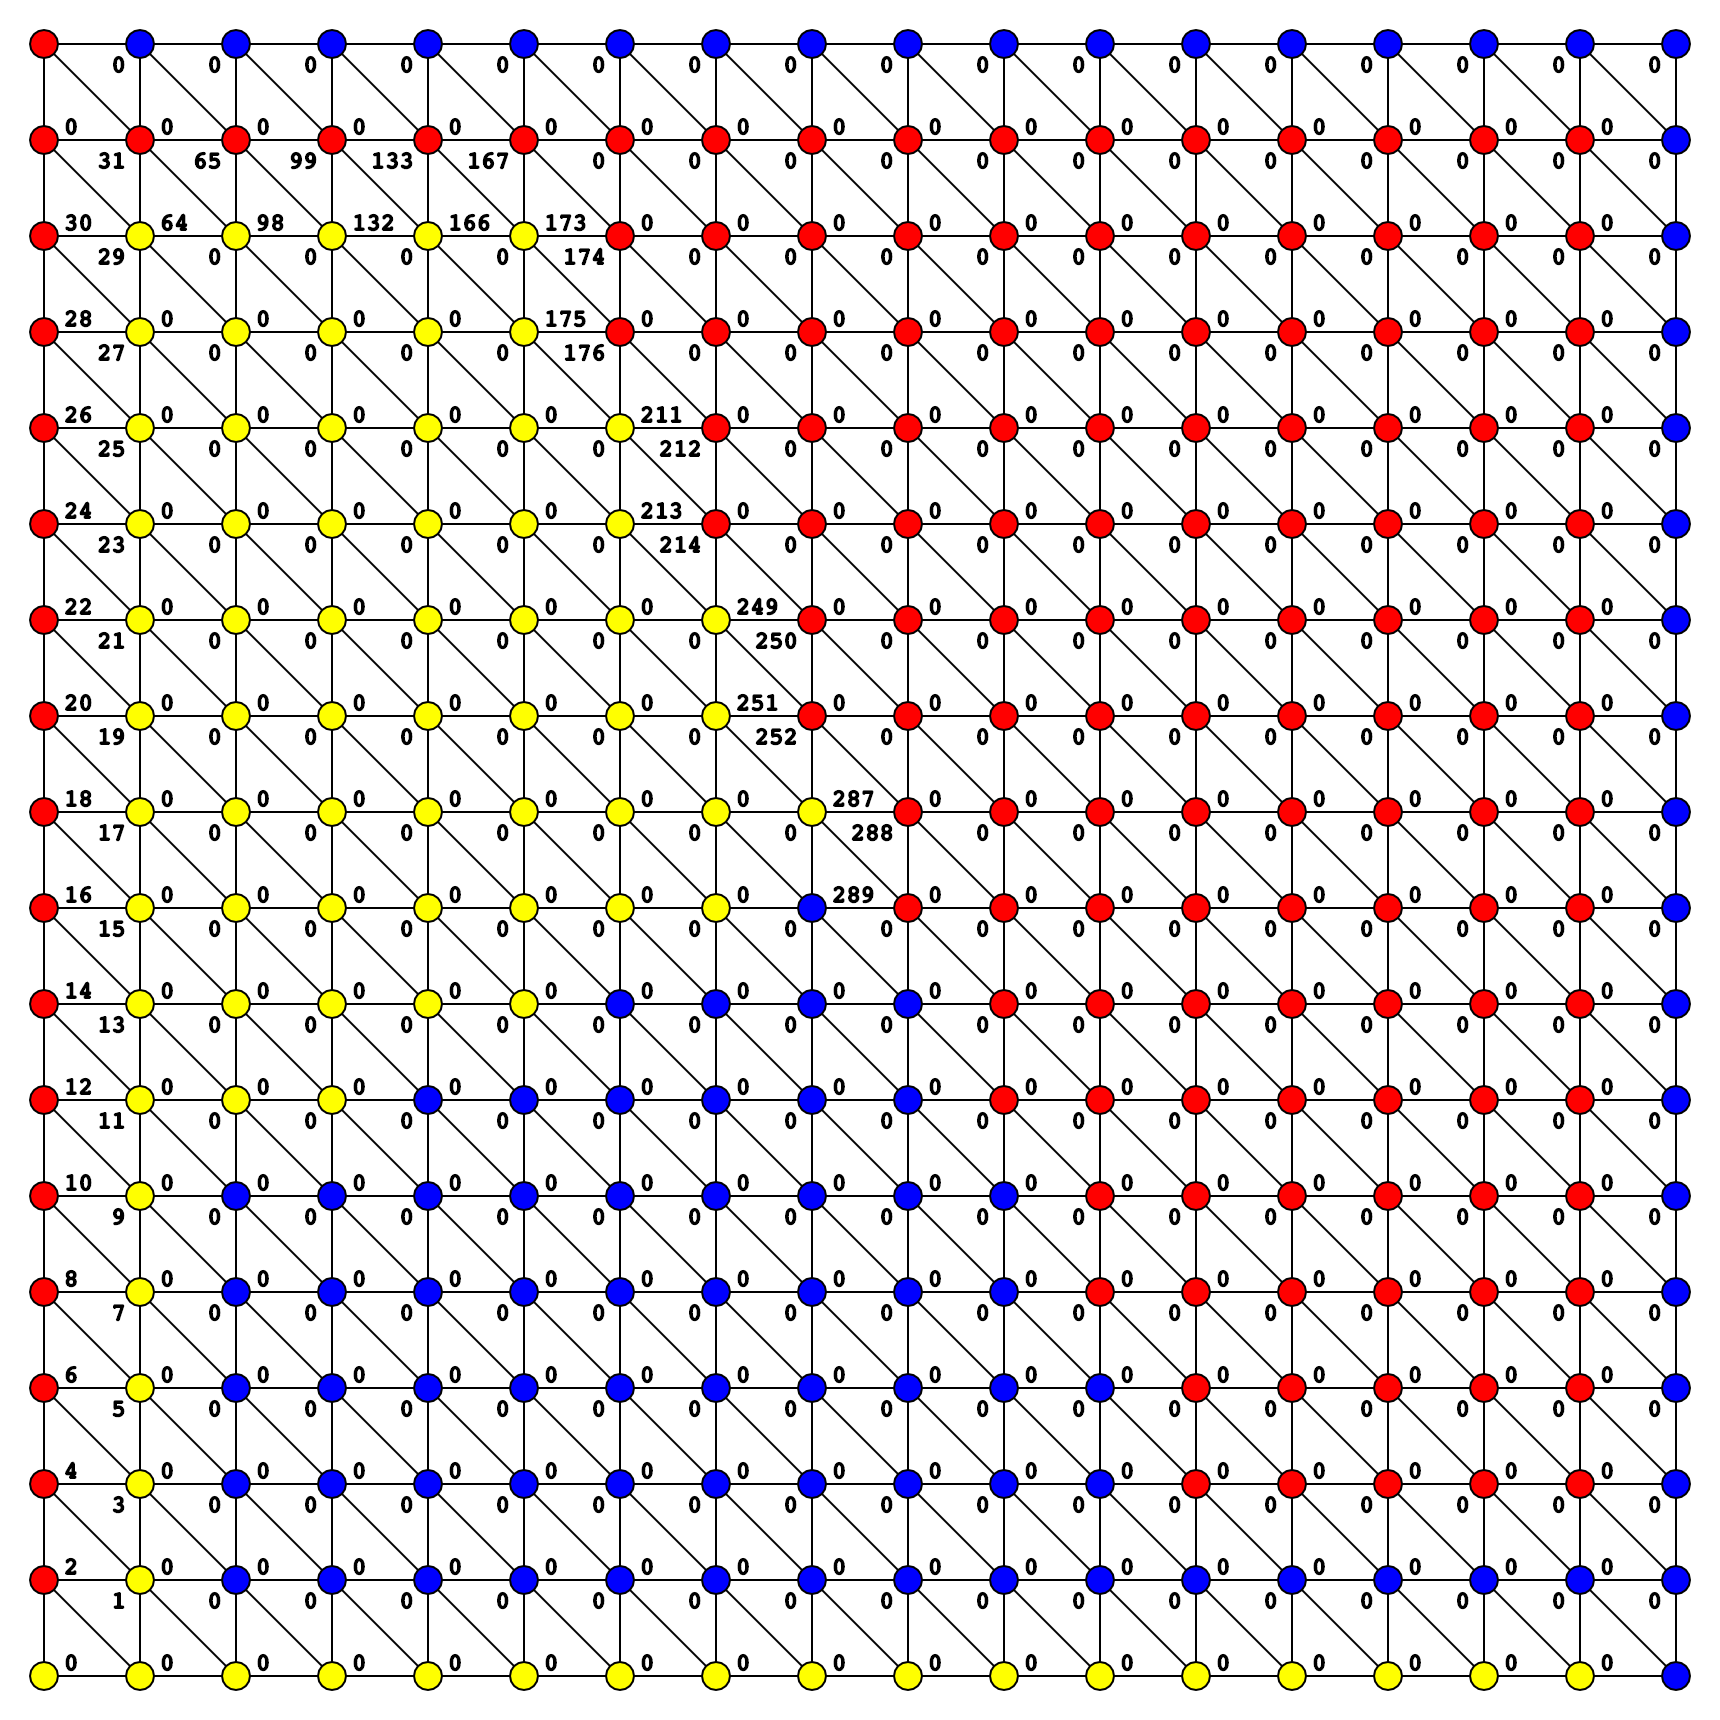
\includegraphics[width=0.9\textwidth]{ContractionToEOPL_example1_potentials}
    \label{fig:potentials}
  \end{figure}

  \begin{lemma} \label{lemma:PotentialsIncreaseAlongPaths}
    For any triangles $T_1,T_2 \in \Delta(\Dom)$ with $T_1 \neq T_2$, if $\Succ(T_1) = T_2$ and $\Pred(T_2) = T_1$, then $\Value(T_1) < \Value(T_2)$. 
  \end{lemma}

  \begin{proof}
    Since $T_1$ and $T_2$ are adjacent in the \EOPL graph, they must share a side. Furthermore, $T_2$ cannot be to the left of $T_1$ since we break all paths rather than introduce an edge to the left. Thus, there are three cases to consider:
    \begin{description}
    \item[$T_2$ is above $T_1$] In this case, the potential at $T_2$ and $T_1$ will be computed counting from the bottom of the column, and $\Value(T_2) > \Value(T_1)$.
    \item[$T_2$ is below $T_1$] In this case, the potential at $T_2$ and $T_1$ will be computed counting from the top of the column and $\Value(T_2) > \Value(T_1)$. 
    \item[$T_2$ is to the right of $T_1$] The potential of any triangle (with non-zero potential) in a given column will be greater than the potential of any triangle in any column to the left of the given column. Thus, $\Value(T_2) > \Value(T_1)$.
    \end{description}
  \end{proof}

  As a corollary of the above lemma, we get

  \begin{corollary} \label{coro:BadPotentialGiveViolations}
    There are no solutions of type \ref{eopl2:bad_potential} in the instance $\CE$ generated by our reduction.
  \end{corollary}

  \begin{lemma} \label{lemma:EndOfLineSolutions}
    Any solution $T \in \Delta(\Dom)$ of type \ref{eopl2:eol} gives a solution for the \TwoDContractionMap instance.
  \end{lemma}
  \begin{proof}
     Consider a solution $T \in \Delta(\DomInt)$ of type \ref{eopl2:eol}. By construction, every triangle without a red-yellow side is in a self-loop, so $T$ must have at least one red vertex and at least one yellow vertex. There are two cases to consider: Either $T$ also has a blue vertex, in which it is a trichromatic triangle, and gives a solution of type \ref{2dcm:fixpoint} by Lemma \ref{lemma:TrichromaticTriangles}, or two of $T$'s vertices are either red or yellow. In the latter case, one of the red-yellow sides must not correspond to a valid edge in the graph, since $T$ is the either the start or end of a line. The only red-yellow sides that don't correspond to valid edges in the graph are those that are predecessor edges to the right, or successor edges to the left. In either of those case, there is a yellow vertex above a red vertex in $T$, and by Lemma \ref{lemma:YellowAboveRed}, the yellow and red vertices witness $f$ not being a contraction map, and give a solution of type \ref{2dcm:violation}.
    \end{proof}
    
    To complete the reduction, we choose for our starting triangle the following: \[(-1/n,0),(0,-1/n),(-1/n,-1/n).\] We can immediately observe that this satisfies the requirement that it has no valid predecessor.

    Finally, we observe that all of the algorithms presented can be implemented in polynomial time in the size of the input to $\CI$, and we conclude that
    \begin{theorem}
An instance of \TwoDContractionMap can be reduced to an instance of \EOPL in polynomial time such that a solution of the former can be constructed in polynomial time from the solution of the latter. 
    \end{theorem}

    
  
  % \begin{enumerate}
  % \item As far as I can tell, there can be edges pointing up in the graph other than those induced by the boundary. I should come up with an example containing edges of that sort. 
  % \item I believe this can be generalized to \ThreeDContractionMap, since I think it will be the case that paths will be limited in a similar way, so that we can assign consistent potential values to each point. 
  % \item We can look at the DTZ paper and see if their hardness proof gives us a metric from which we could do this same reduction. Or we could modify their metric somehow and still carry out the same sort of proof.
  % Can we use the $\lambda$-Lipschitz continuity of $d$ in the DTZ definition of MetricBanach to generalize this argument to that definition. 

  % If it's the case that we're given a metric which is of the form $d(x,y) = g(\Abs{x_1-x_2},\Abs{y_1-y_2})$, where $g$ is a non-decreasing function in both arguments, then I think everything works out. We may be able to extract solutions from violations of this. (Probably not, seems too rigid a constraint.)

  % Fix the JavaScript to make sure all the colors are being computed correctly, and then update the images accordingly.

  % \end{enumerate}

  % One other interesting observation: When $f$ is in fact a contraction map, there can be at most one edge from left-to-right in any given column by Lemma \ref{lemma:YellowAboveRed}. 

  % Can we go from EOPL to a standard norm-based contraction in $n$-dimensions?

  % What is the role of uniqueness of solutions.
  